\section{Interfaccia grafica}
Questa sezione è dedicata all'interfaccia grafica dell'applicazione OpenLDAT, implementata nel package \texttt{com.dosse.openldat.ui}.

L'interfaccia è stata sviluppata utilizzando le librerie Swing di Java SE con alcuni accorgimenti per supportare i display con DPI alti, e permette di avviare i test e visualizzarne i risultati in maniera semplice e intuitiva. Non c'è nulla di particolarmente interessante dal punto di vista tecnico nell'implementazione della GUI, per cui questa sezione si concentra principalmente sulle funzionalità e l'utilizzo dell'interfaccia grafica.

Attualmente non sono implementate localizzazioni, l'interfaccia è disponibile solo in lingua Inglese.

L'interfaccia è pensata per essere utilizzata con un mouse, ma è presente un supporto limitato per i touchscreen e la navigazione da tastiera.

\subsection{Selezione del dispositivo}
All'avvio dell'applicazione viene scansionato il PC per trovare dispositivi OpenLDAT connessi. Se viene trovato più di un dispositivo, viene mostrata una schermata di selezione come quella in figura \ref{fig:gui_deviceSelector} da cui è possibile distinguerli in base alla porta a cui sono collegati. Se c'è un solo dispositivo questa schermata viene saltata.

\begin{figure}[h]
	\centering
	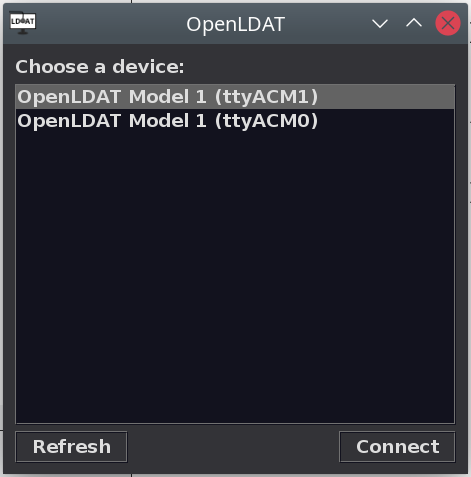
\includegraphics[width=.5\textwidth]{Chapter04/res/gui_deviceSelector.png}
	\caption{Selezione del dispositivo}
	\label{fig:gui_deviceSelector}
\end{figure}

Premendo il pulsante Connect si avvia l'applicazione utilizzando il dispositivo selezionato, premendo Refresh è possibile rieseguire la scansione.

\subsection{Menu principale}
Dopo la selezione del dispositivo, viene visualizzato il menu principale dell'applicazione come in figura \ref{fig:gui_mainMenu2}. Questa schermata è divisa in due parti: a sinistra sono elencati tutti i test e le funzioni dell'applicazione, sulla destra è presente un manuale che mostra informazioni sul test selezionato e il pulsante per avviarlo. Le pagine del manuale mostrato sulla destra sono memorizzate come dei file HTML nella cartella \texttt{manual} all'interno del package della GUI.

\begin{figure}[h]
	\centering
	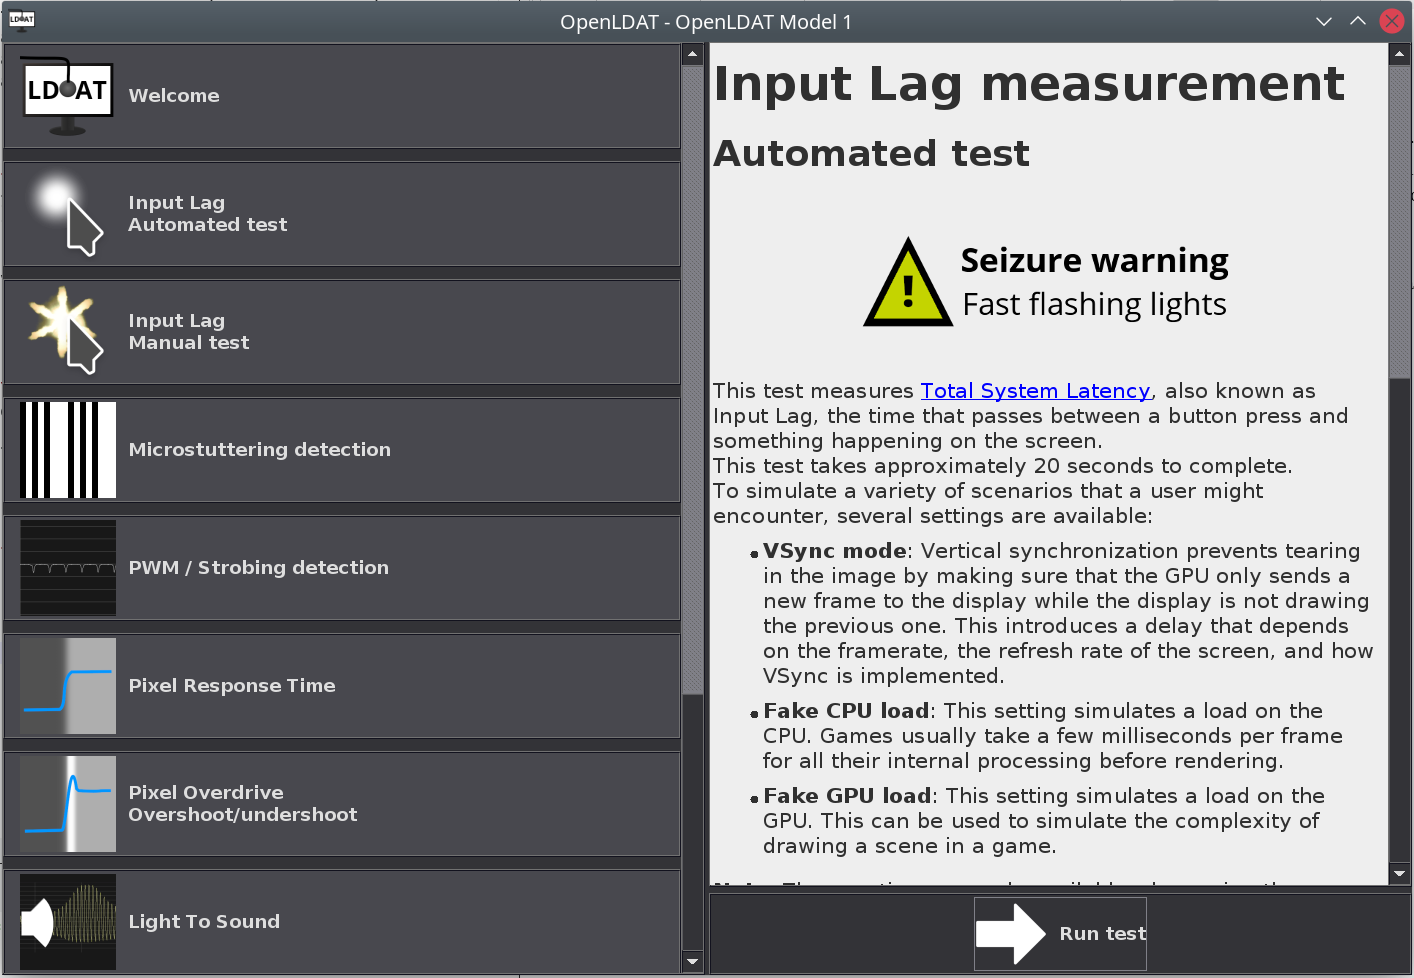
\includegraphics[width=\textwidth]{Chapter04/res/gui_mainMenu2.png}
	\caption{Menu principale con un test selezionato}
	\label{fig:gui_mainMenu2}
\end{figure}

Il menu principale fornisce accesso alle seguenti funzioni:\begin{itemize}
	\item \textbf{Welcome}: mostra una schermata di benvenuto con alcuni suggerimenti generali per l'utilizzo corretto dei test
	\item \textbf{Input Lag (Automated test)}: esegue il test automatico del ritardo di input
	\item \textbf{Input Lag (Manual test)}: esegue il test interattivo del ritardo di input
	\item \textbf{Microstuttering detection}: esegue il test di rilevamento del microstuttering
	\item \textbf{PWM/Strobing test}: esegue il test di rilevamento PWM e altri rumori
	\item \textbf{Pixel Response Time}: esegue il test che misura il tempo di risposta dei pixel tra diverse sfumature di grigio
	\item \textbf{Pixel Overdrive (Overshoot/Undershoot)}: esegue il test che misura l'errore di transizione causato dall'overdrive dei pixel
	\item \textbf{Light To Sound}: avvia la modalità Light To Sound, per ascoltare i dati catturati dal sensore di luminosità
	\item \textbf{Driver test}: fornsice accesso a un pannello da cui è possibile testare tutte le funzioni del dispositivo, del driver, e del processamento di base
	\item \textbf{Advanced settings}: permette di cambiare alcune impostazioni dell'applicazione che normalmente sono determinate automaticamente
	\item \textbf{About OpenLDAT}: mostra informazioni sull'applicazione
\end{itemize}

\subsection{Test automatici}
I test automatici seguono tutti i seguenti passi quando vengono avviati:\begin{itemize}
	\item Se il test ha dei parametri configurabili, mostra una schermata di configurazione
	\item Esegui il test
	\item Mostra una schermata con i risultati
	\item Torna al menu principale
\end{itemize}

\subsubsection{Input lag (test automatico)}
Questo test ha dei parametri che possono essere configurati, mostrati in figura \ref{fig:gui_inputlag_settings}:\begin{itemize}
	\item \textbf{VSync mode}: permette di attivare o disattivare il VSync
	\item \textbf{Fake CPU load}: simula la presenza di carico sulla CPU durante l'esecuzione del test. Il carico è espresso in millisecondi per frame
	\item \textbf{Fake GPU load}: simula la presenza di carico sulla GPU durante l'esecuzione del test. Il carico è espresso in millisecondi per frame
	\item \textbf{Test duration}: permette di selezionare la durata del test tra 20 secondi, 1 minuto (default), 2 minuti o 5 minuti. Test più lunghi garantiscono risultati più accurati
\end{itemize}

Al termine del test, viene visualizzata una schermata con i risultati come in figura \ref{fig:gui_inputlag_results}. Da quì è possibile salvarli su un file importabile in un foglio di calcolo oppure tornare al menu principale.

\begin{figure}[H]
	\centering
	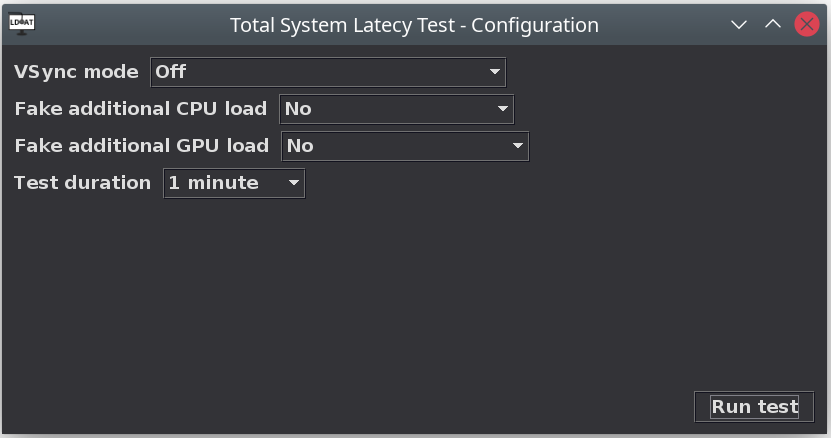
\includegraphics[width=.8\textwidth]{Chapter04/res/gui_inputlag_settings.png}
	\caption{Input lag: impostazioni del test}
	\label{fig:gui_inputlag_settings}
\end{figure}

\begin{figure}[H]
	\centering
	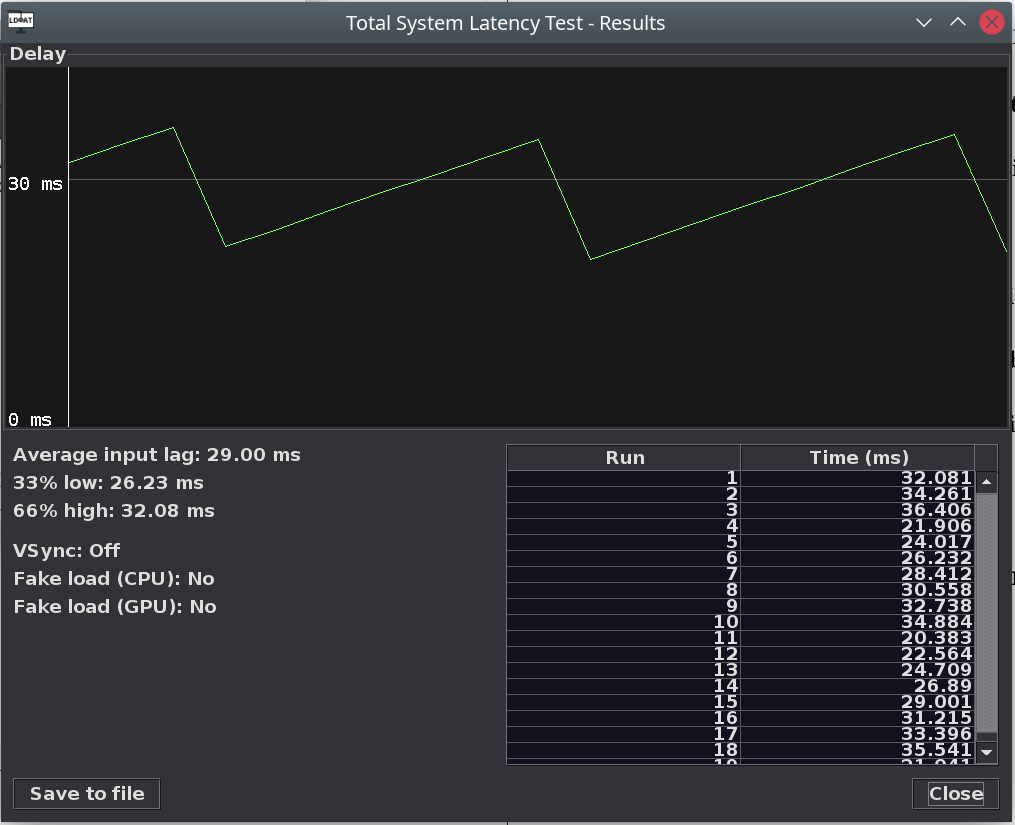
\includegraphics[width=\textwidth]{Chapter04/res/gui_inputlag_results.png}
	\caption{Input lag: risultati del test}
	\label{fig:gui_inputlag_results}
\end{figure}

\subsubsection{Rilevamento del microstuttering}
Questo test non ha parametri da configurare, per cui viene eseguito immediatamente. Al termine viene mostrata una schermata con i risultati come in figura \ref{fig:gui_microstuttering_results}. Da quì è possibile salvarli su un file importabile in un foglio di calcolo oppure tornare al menu principale. La presenza di picchi sopra la linea rossa nel grafico indica la presenza di microstuttering.

Nota: è stato osservato che su alcune piattaforme, il backend Swing, non essendo in grado di sincronizzarsi con il display, può generare esso stesso microstuttering; per questo motivo, al fine di evitare di fornire dati potenzialmente errati, è stato scelto di far funzionare questo test solo con il backend OpenGL. Il codice del test supporta entrambi i backend, la restrizione è presente solo nel codice della GUI che avvia il test.

\begin{figure}[H]
	\centering
	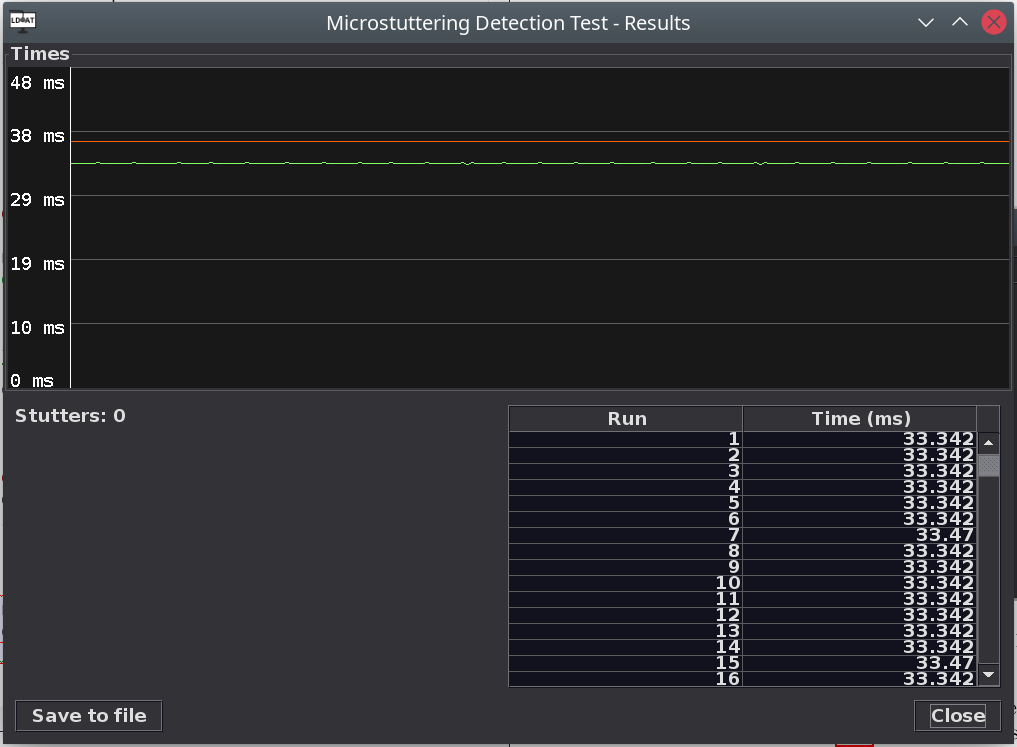
\includegraphics[width=\textwidth]{Chapter04/res/gui_microstuttering_results.png}
	\caption{Rilevamento del microstuttering: risultati del test}
	\label{fig:gui_microstuttering_results}
\end{figure}

\subsubsection{Rilevamento di PWM e noise}
Questo test non ha parametri da configurare, per cui viene eseguito immediatamente. Al termine viene mostrata una schermata con i risultati come in figura \ref{fig:gui_pwm_results}. Da quì è possibile salvarli su un file importabile in un foglio di calcolo oppure tornare al menu principale. Il grafico mostra il segnale catturato dal sensore durante il test.

\begin{figure}[H]
	\centering
	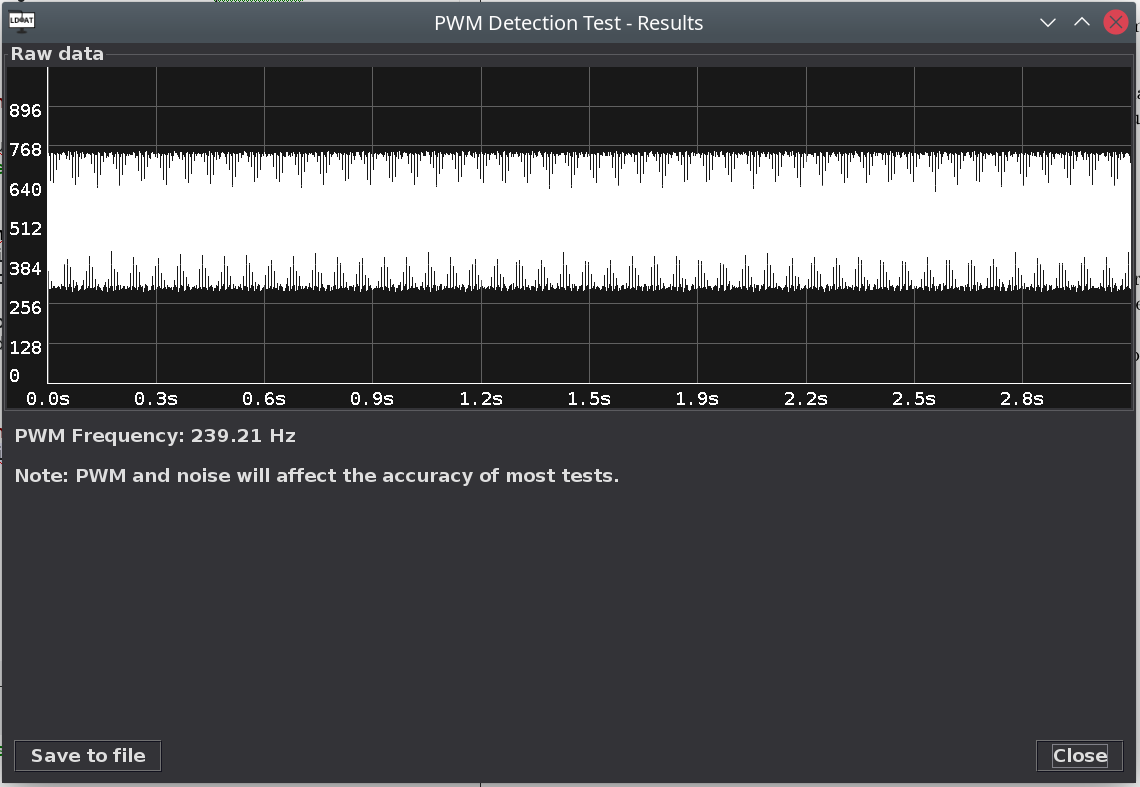
\includegraphics[width=\textwidth]{Chapter04/res/gui_pwm_results.png}
	\caption{Rilevamento di PWM e noise: risultati del test su un display con una pessima retroilluminazione}
	\label{fig:gui_pwm_results}
\end{figure}

\subsubsection{Tempi di risposta dei pixel}
Questo test ha due parametri che possono essere configurati, mostrati in figura \ref{fig:gui_pixelresponse_settings}:\begin{itemize}
	\item \textbf{Evaluation method}: permette di scegliere il range della transizione di cui misurare il tempo. Lo standard VESA prevede di misurare il tempo richiesto per la transizione dal 10\% al 90\%, per cui questo è il default, ma può essere selezionata anche un'altra modalità chiamata umoristicamente "BS Manufactures Say" per misurare il range 30\%-70\%, che è più tipicamente usato dai produttori di schermi "da gaming"
	\item \textbf{Step size}: il passo tra due sfumature di grigio. Valori più piccoli testano più sfumature di grigio ma rendono il test molto più lungo. I valori implementati sono 16 (lento), 32 (default) e 64 (veloce). Questi valori sono su una scala tra 0 e 255 solo per comodità, il test utilizza il formato dei pixel del desktop
\end{itemize}

Al termine del test, viene visualizzata una schermata con i risultati come in figura \ref{fig:gui_pixelresponse_results}. Da quì è possibile salvarli su un file importabile in un foglio di calcolo oppure tornare al menu principale. I colori nella tabella indicano in modo intuitivo quanto è buono il tempo di quella transizione con una sfumatura dal verde al rosso.

Nota: i valori di luminosità sono su una scala tra 0 e 255 solo per comodità, il test utilizza il formato dei pixel del desktop.

\begin{figure}[H]
	\centering
	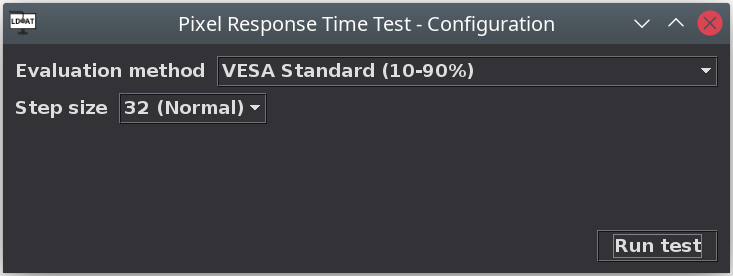
\includegraphics[width=.8\textwidth]{Chapter04/res/gui_pixelresponse_settings.png}
	\caption{Tempi di risposta dei pixel: impostazioni del test}
	\label{fig:gui_pixelresponse_settings}
\end{figure}

\begin{figure}[H]
	\centering
	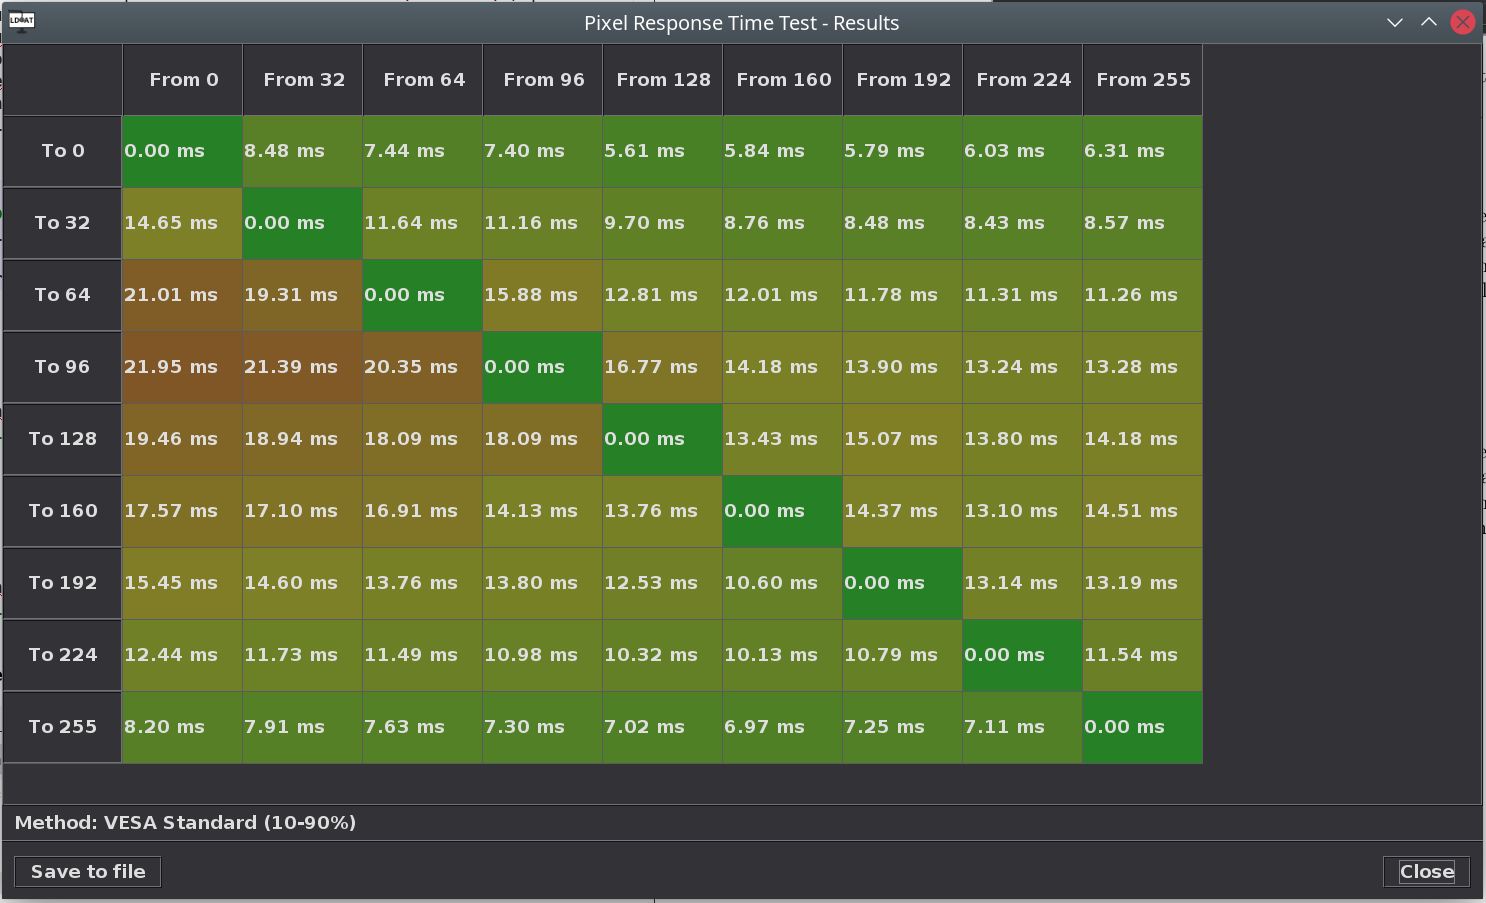
\includegraphics[width=\textwidth]{Chapter04/res/gui_pixelresponse_results.png}
	\caption{Tempi di risposta dei pixel: risultati del test}
	\label{fig:gui_pixelresponse_results}
\end{figure}

\subsubsection{Overdrive dei pixel}
Questo test ha tre parametri che possono essere configurati, mostrati in figura \ref{fig:gui_pixeloverdrive_settings}:\begin{itemize}
	\item \textbf{Method}: permette di scegliere il metodo di misurazione tra Relativo e Assoluto (default), il cui significato è approfondito nella sezione dedicata al funzionamento di questo test
	\item \textbf{Step size}: il passo tra due sfumature di grigio. Valori più piccoli testano più sfumature di grigio ma rendono il test molto più lungo. I valori implementati sono 16 (lento), 32 (default) e 64 (veloce). Questi valori sono su una scala tra 0 e 255 solo per comodità, il test utilizza il formato dei pixel del desktop
	\item \textbf{Skip transitions to 0 and 255}: velocizza il test saltando le transizioni verso il nero e verso il bianco, dato che normalmente il display non può visualizzare colori più scuri del nero o più chiari del bianco
\end{itemize}

Al termine del test, viene visualizzata una schermata con i risultati come in figura \ref{fig:gui_pixeloverdrive_results}. Da quì è possibile salvarli su un file importabile in un foglio di calcolo oppure tornare al menu principale. I colori nella tabella indicano in modo intuitivo quanto è buono il tempo di quella transizione con una sfumatura dal verde al rosso.

Attenzione: questo test è estremamente sensibile alla presenza di PWM o altri disturbi.

Nota: i valori di luminosità sono su una scala tra 0 e 255 solo per comodità, il test utilizza il formato dei pixel del desktop.

\begin{figure}[H]
	\centering
	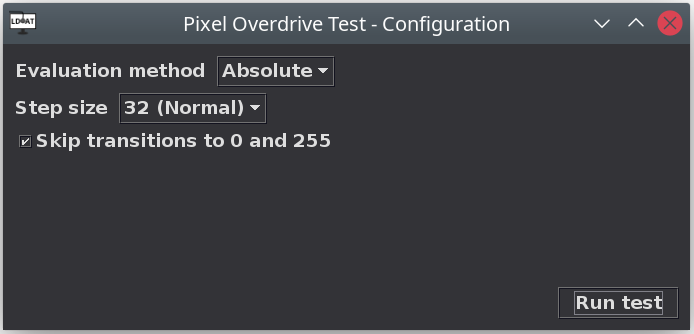
\includegraphics[width=.8\textwidth]{Chapter04/res/gui_pixeloverdrive_settings.png}
	\caption{Overdrive dei pixel: impostazioni del test}
	\label{fig:gui_pixeloverdrive_settings}
\end{figure}

\begin{figure}[H]
	\centering
	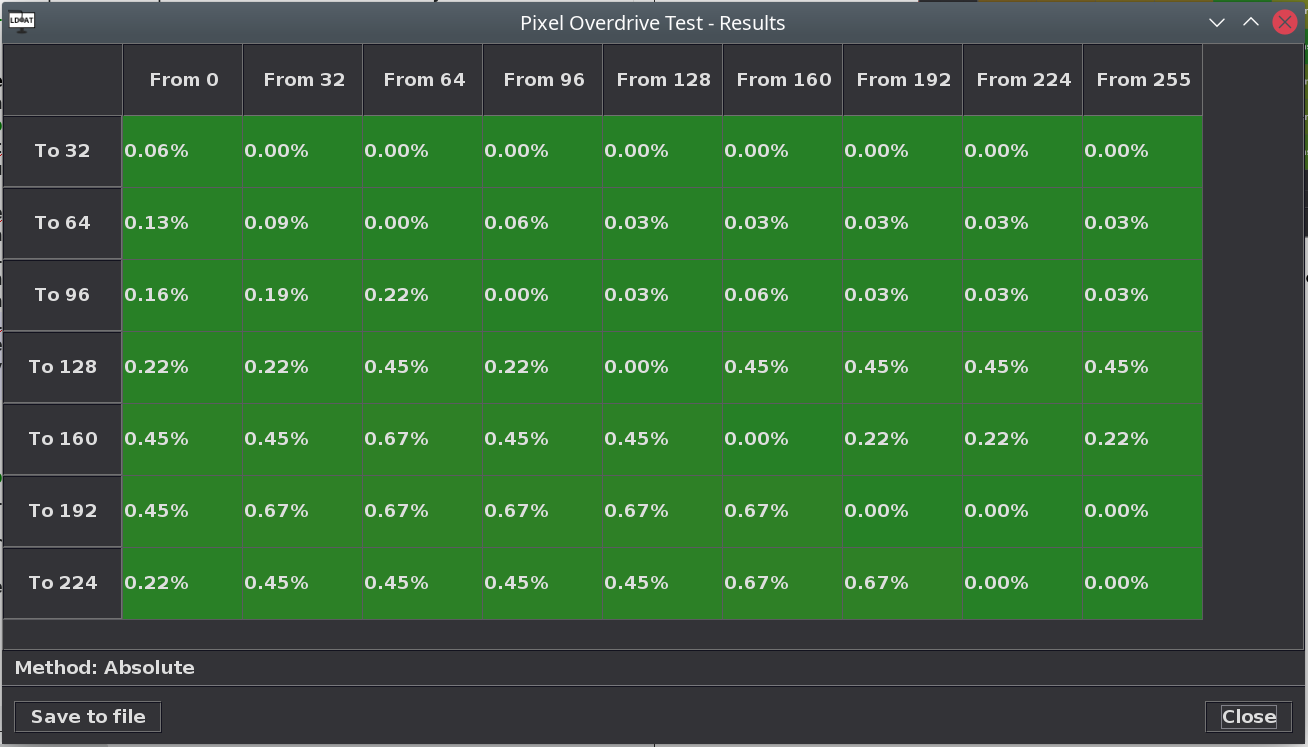
\includegraphics[width=\textwidth]{Chapter04/res/gui_pixeloverdrive_results.png}
	\caption{Overdrive dei pixel: risultati del test}
	\label{fig:gui_pixeloverdrive_results}
\end{figure}

\subsection{Test interattivi}
I test interattivi mostrano una schermata di test in cui è possibile configurarlo mentre il test è in esecuzione. Questi test procedono indefinitamente fino a quando non vengono interrotti dall'utente.

\subsubsection{Input lag (test interattivo)}
Questo test permette di misurare il ritardo in risposta ai click di virtualmente qualsiasi applicazione.

L'interfaccia grafica del test (figura \ref{fig:gui_interactiveinputlag_results}) è organizzata in questo modo:\begin{itemize}
	\item Il grafico mostra i dati del sensore di luminosità (bianco), i click (azzurro), e la soglia di attivazione (linea verde orizzontale)
	\item Alla destra del grafico è possibile regolare la soglia di attivazione con il cursore
	\item Sotto al grafico, sulla destra è possibile cambiare il gain del sensore tra i quattro livelli disponibili e scegliere se i click devono essere generati automaticamente dal dispositivo o se devono essere ricevuti dall'esterno (default)
	\item Sotto al grafico, a sinistra è presente un elenco di tempi misurati finora con la relativa media e la possibilità di salvare i tempi su file e di resettare il test qualora siano stati catturati dati errati
\end{itemize}

\begin{figure}[H]
	\centering
	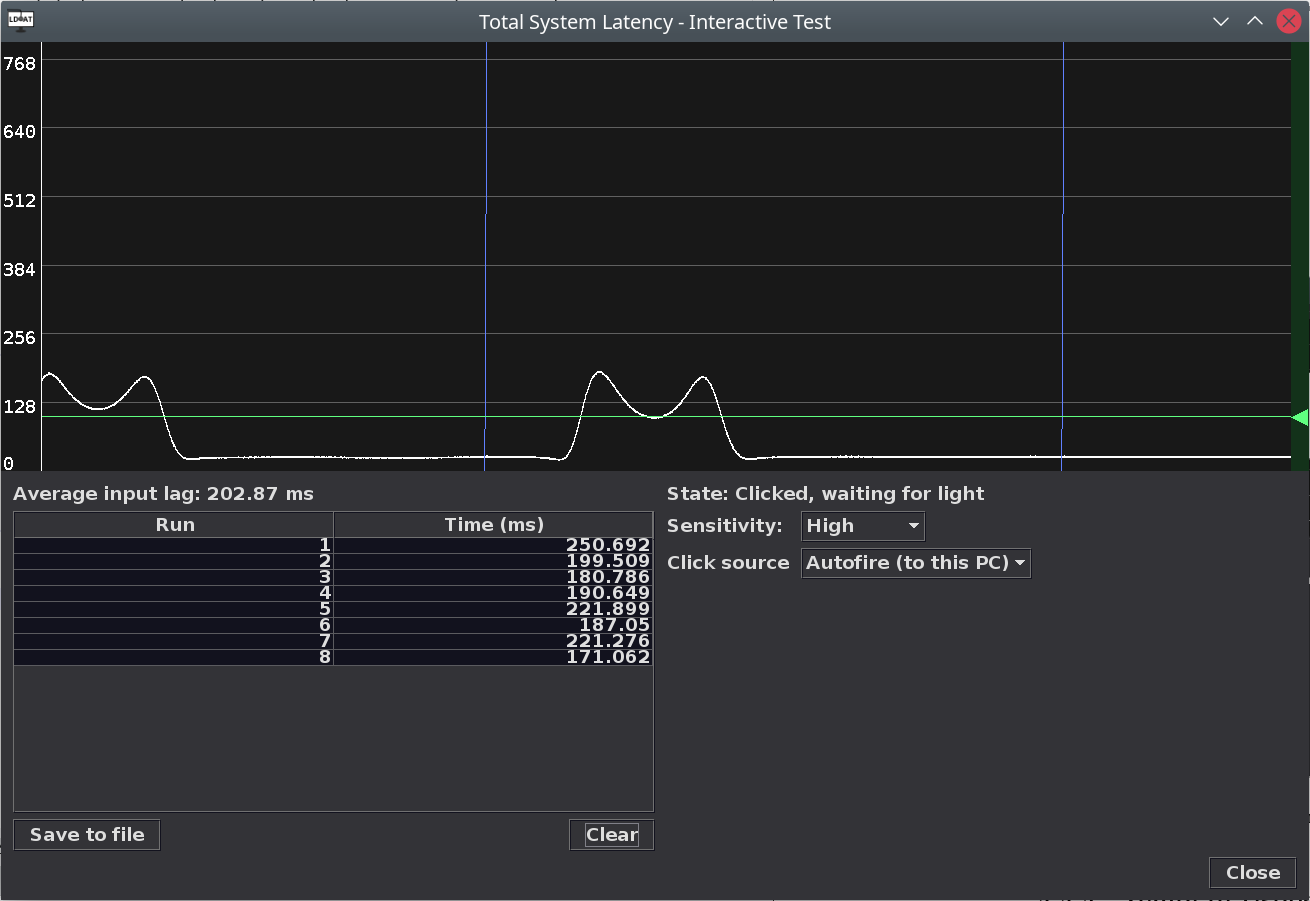
\includegraphics[width=\textwidth]{Chapter04/res/gui_interactiveinputlag_results.png}
	\caption{Input lag (test interattivo): schermata di test}
	\label{fig:gui_interactiveinputlag_results}
\end{figure}

\subsubsection{Light to sound}
Quest'ultimo test permette di ascoltare il segnale del sensore di luminosità come audio.

L'interfaccia grafica del test (figura \ref{fig:gui_lighttosound_results}) è organizzata in questo modo:\begin{itemize}
	\item Il grafico mostra l'ultimo mezzo secondo del segnale catturato
	\item I controlli sotto al grafico permettono di regolare il volume dell'audio e il livello di gain del sensore
	\item Quando viene rilevata una frequenza sufficientemente potente (ad esempio da una retroilluminazione PWM), questa viene mostrata sotto ai controlli
	\item In basso a sinistra viene mostrato il sample rate del segnale catturato
\end{itemize}

\begin{figure}[H]
	\centering
	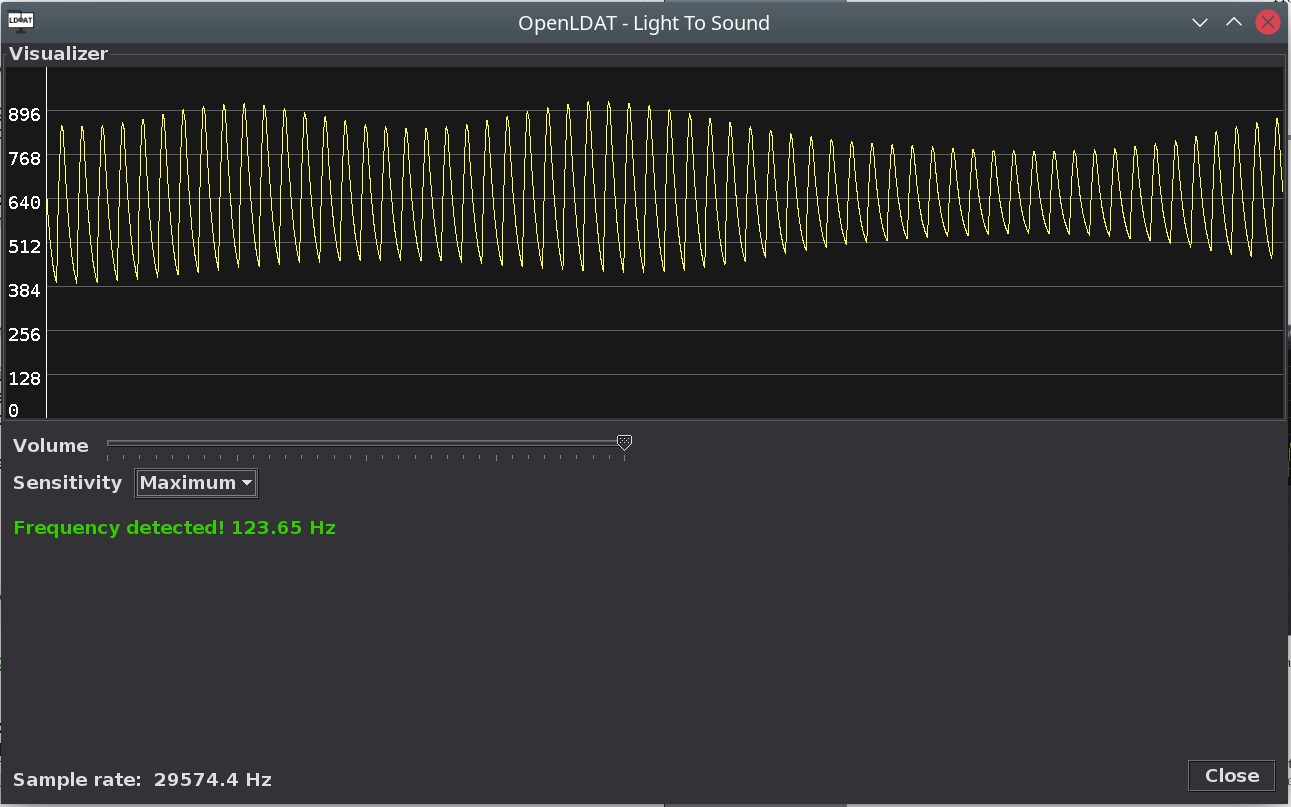
\includegraphics[width=\textwidth]{Chapter04/res/gui_lighttosound_results.png}
	\caption{Light to sound: schermata di test}
	\label{fig:gui_lighttosound_results}
\end{figure}

\subsection{Impostazioni}
La schermata delle impostazioni mostrata in figura \ref{fig:gui_settings} permette di cambiare alcune impostazioni che l'applicazione determina automaticamente:\begin{itemize}
	\item \textbf{Graphics backend}: seleziona il backend grafico tra OpenGL e Swing. Di default viene usato OpenGL se è disponibile, Swing è usato solo come fallback
	\item \textbf{Use antialiasing on charts (slower)}: migliora la qualità dei grafici disegnandoli con l'antialiasing. Di default è disattivato
	\item \textbf{Disable X11 hacks}: permette di disattivare alcuni hack che aumentano la stabilità dell'applicazione su X11 (solo per GNU/Linux). Di default è disattivato
\end{itemize}

Queste impostazioni sono rese disponibili a tutte le classi dell'applicazione sotto forma di variabili statiche nella classe \texttt{Config}, la quale si occupa anche di memorizzarle su disco e applicarle anche ai successivi utilizzi. Le impostazioni sono memorizzate nella cartella \texttt{\textasciitilde/.openldat} (GNU/Linux e MacOS) o \texttt{\%USERPROFILE\%\textbackslash.openldat} (Windows).

\begin{figure}[H]
	\centering
	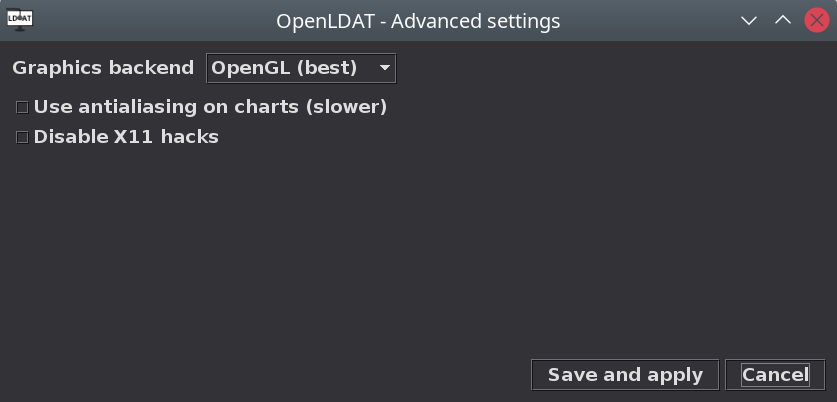
\includegraphics[width=\textwidth]{Chapter04/res/gui_settings.png}
	\caption{Impostazioni dell'applicazione}
	\label{fig:gui_settings}
\end{figure}

\subsection{Schermata about}
Questa schermata mostra le informazioni sull'applicazione: versione, copyright e licenza (GNU GPL Versione 3).

\begin{figure}[H]
	\centering
	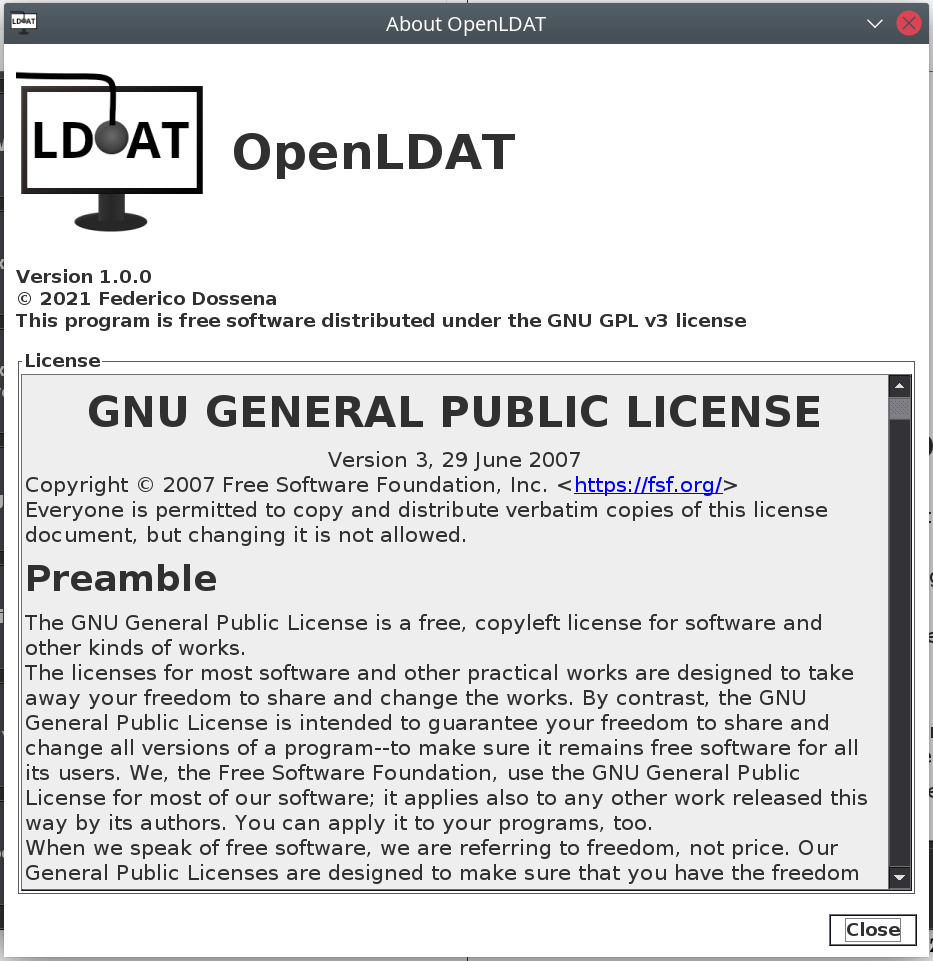
\includegraphics[width=.8\textwidth]{Chapter04/res/gui_about.png}
	\caption{Informazioni su OpenLDAT}
	\label{fig:gui_about}
\end{figure}

Facendo click ripetutamente sul logo di OpenLDAT per 7 volte è possibile accedere al Driver test anche su dispositivi che non sono marcati come prototipi.

\subsection{Gestore grafico degli errori}
L'ultimo componente della GUI è il gestore degli errori. La classe \texttt{ErrorDialog} implementa la schermata di errore in figura \ref{fig:gui_errordialog} e può gestire i seguenti errori:\begin{itemize}
	\item \textbf{Errori dell'applicazione}: file corrotti, applicazione già avviata, crash di thread, eccetera. Questi errori sono critici e causano la chiusura dell'applicazione
	\item \textbf{Errori del dispositivo e del driver}: dispositivi non supportati, disconnessioni inaspettate, risposte non valide del firmware, eccetera. Questi errori sono critici e causano la chiusura dell'applicazione
	\item \textbf{Errori dei test}: fallimenti nell'analisi, contrasto insufficiente, problemi con il backend grafico, sensori mancanti, eccetera. Questi errori causano il fallimento del test, ma l'applicazione può continuare. Alcuni di questi errori, per esempio l'annullamento del test da parte dell'utente, non causano la visualizzazione di un messaggio d'errore
\end{itemize}

\begin{figure}[H]
	\centering
	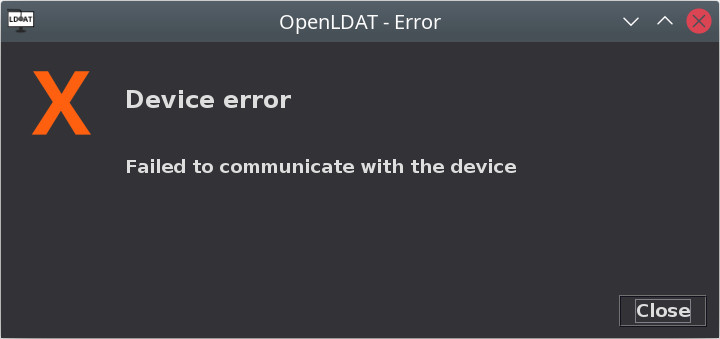
\includegraphics[width=.8\textwidth]{Chapter04/res/gui_errordialog.png}
	\caption{Schermata di errore di OpenLDAT}
	\label{fig:gui_errordialog}
\end{figure}

Un errore che viene trattato in modo speciale da questa classe è quello che si verifica se il dispositivo viene rilevato ma l'utente corrente non ha i permessi per comunicare con esso. Questo è un problema che si verifica su alcune distribuzioni di GNU/Linux e l'applicazione implementa una schermata di errore speciale (figura \ref{fig:gui_linuxerror}) che si offre di correggere i permessi automaticamente tramite uno script (se l'utente è amministratore) o di mostrare istruzioni su come farlo manualmente da un terminale.\\
Lo script automatico supporta distribuzioni GNU/Linux basate su Debian, Arch, SUSE e RedHat, ed è stato testato su Ubuntu 21.04, Debian 10.9, Manjaro 21, Arch Linux (Aprile 2021), OpenSUSE 15, Fedora 34.

\begin{figure}[H]
	\centering
	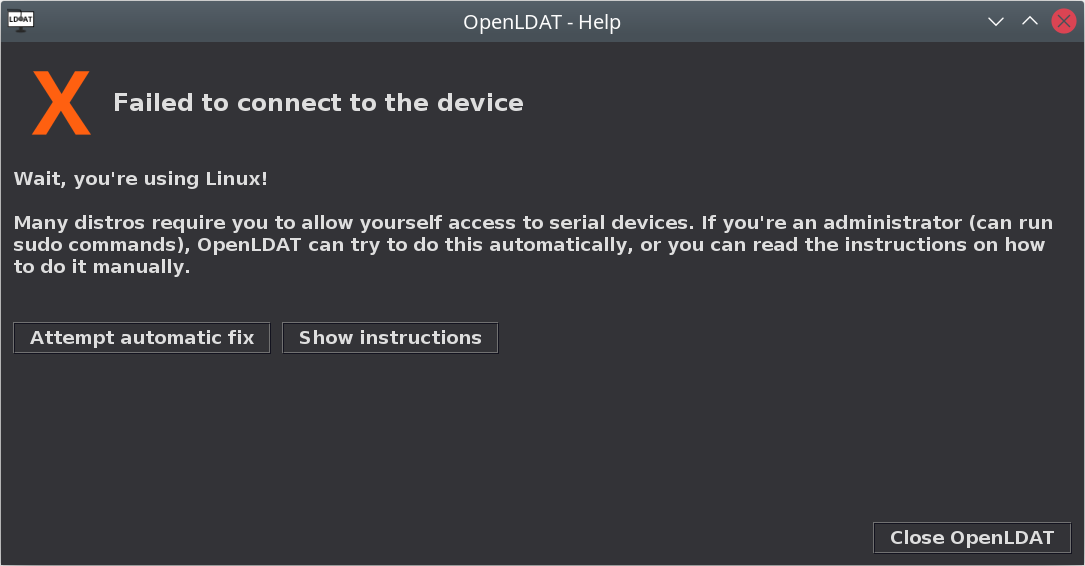
\includegraphics[width=\textwidth]{Chapter04/res/gui_linuxerror.png}
	\caption{Correzione automatica dei permessi mancanti su GNU/Linux}
	\label{fig:gui_linuxerror}
\end{figure}

Questo conclude la sezione di presentazione dell'interfaccia grafica dell'applicazione OpenLDAT.